\documentclass[12pt, a4paper]{article}

%<*preamble>
% Math symbols
\usepackage{amsmath, amsthm, amsfonts, amssymb}
\usepackage{accents}
\usepackage{esvect}
\usepackage{mathrsfs}
\usepackage{mathtools}
\mathtoolsset{showonlyrefs}
\usepackage{cmll}
\usepackage{stmaryrd}
\usepackage{physics}
\usepackage[normalem]{ulem}
\usepackage{ebproof}
\usepackage{extarrows}

% Page layout
\usepackage{geometry, a4wide, parskip, fancyhdr}

% Font, encoding, russian support
\usepackage[russian]{babel}
\usepackage[sb]{libertine}
\usepackage{xltxtra}

% Listings
\usepackage{listings}
\lstset{basicstyle=\ttfamily,breaklines=true}
\setmonofont{Inconsolata}

% Miscellaneous
\usepackage{array}
\usepackage{calc}
\usepackage{caption}
\usepackage{subcaption}
\captionsetup{justification=centering,margin=2cm}
\usepackage{catchfilebetweentags}
\usepackage{enumitem}
\usepackage{etoolbox}
\usepackage{float}
\usepackage{lastpage}
\usepackage{minted}
\usepackage{svg}
\usepackage{wrapfig}
\usepackage{xcolor}
\usepackage[makeroom]{cancel}

\newcolumntype{L}{>{$}l<{$}}
    \newcolumntype{C}{>{$}c<{$}}
\newcolumntype{R}{>{$}r<{$}}

% Footnotes
\usepackage[hang]{footmisc}
\setlength{\footnotemargin}{2mm}
\makeatletter
\def\blfootnote{\gdef\@thefnmark{}\@footnotetext}
\makeatother

% References
\usepackage{hyperref}
\hypersetup{
    colorlinks,
    linkcolor={blue!80!black},
    citecolor={blue!80!black},
    urlcolor={blue!80!black},
}

% tikz
\usepackage{tikz}
\usepackage{tikz-cd}
\usetikzlibrary{arrows.meta}
\usetikzlibrary{decorations.pathmorphing}
\usetikzlibrary{calc}
\usetikzlibrary{patterns}
\usepackage{pgfplots}
\pgfplotsset{width=10cm,compat=1.9}
\newcommand\irregularcircle[2]{% radius, irregularity
    \pgfextra {\pgfmathsetmacro\len{(#1)+rand*(#2)}}
    +(0:\len pt)
    \foreach \a in {10,20,...,350}{
            \pgfextra {\pgfmathsetmacro\len{(#1)+rand*(#2)}}
            -- +(\a:\len pt)
        } -- cycle
}

\providetoggle{useproofs}
\settoggle{useproofs}{false}

\pagestyle{fancy}
\lfoot{M3137y2019}
\cfoot{}
\rhead{стр. \thepage\ из \pageref*{LastPage}}

\newcommand{\R}{\mathbb{R}}
\newcommand{\Q}{\mathbb{Q}}
\newcommand{\Z}{\mathbb{Z}}
\newcommand{\B}{\mathbb{B}}
\newcommand{\N}{\mathbb{N}}
\renewcommand{\Re}{\mathfrak{R}}
\renewcommand{\Im}{\mathfrak{I}}

\newcommand{\const}{\text{const}}
\newcommand{\cond}{\text{cond}}

\newcommand{\teormin}{\textcolor{red}{!}\ }

\DeclareMathOperator*{\xor}{\oplus}
\DeclareMathOperator*{\equ}{\sim}
\DeclareMathOperator{\sign}{\text{sign}}
\DeclareMathOperator{\Sym}{\text{Sym}}
\DeclareMathOperator{\Asym}{\text{Asym}}

\DeclarePairedDelimiter{\ceil}{\lceil}{\rceil}

% godel
\newbox\gnBoxA
\newdimen\gnCornerHgt
\setbox\gnBoxA=\hbox{$\ulcorner$}
\global\gnCornerHgt=\ht\gnBoxA
\newdimen\gnArgHgt
\def\godel #1{%
    \setbox\gnBoxA=\hbox{$#1$}%
    \gnArgHgt=\ht\gnBoxA%
    \ifnum     \gnArgHgt<\gnCornerHgt \gnArgHgt=0pt%
    \else \advance \gnArgHgt by -\gnCornerHgt%
    \fi \raise\gnArgHgt\hbox{$\ulcorner$} \box\gnBoxA %
    \raise\gnArgHgt\hbox{$\urcorner$}}

% \theoremstyle{plain}

\theoremstyle{definition}
\newtheorem{theorem}{Теорема}
\newtheorem*{definition}{Определение}
\newtheorem{axiom}{Аксиома}
\newtheorem*{axiom*}{Аксиома}
\newtheorem{lemma}{Лемма}

\theoremstyle{remark}
\newtheorem*{remark}{Примечание}
\newtheorem*{exercise}{Упражнение}
\newtheorem{corollary}{Следствие}[theorem]
\newtheorem*{statement}{Утверждение}
\newtheorem*{corollary*}{Следствие}
\newtheorem*{example}{Пример}
\newtheorem{observation}{Наблюдение}
\newtheorem*{prop}{Свойства}
\newtheorem*{obozn}{Обозначение}

% subtheorem
\makeatletter
\newenvironment{subtheorem}[1]{%
    \def\subtheoremcounter{#1}%
    \refstepcounter{#1}%
    \protected@edef\theparentnumber{\csname the#1\endcsname}%
    \setcounter{parentnumber}{\value{#1}}%
    \setcounter{#1}{0}%
    \expandafter\def\csname the#1\endcsname{\theparentnumber.\Alph{#1}}%
    \ignorespaces
}{%
    \setcounter{\subtheoremcounter}{\value{parentnumber}}%
    \ignorespacesafterend
}
\makeatother
\newcounter{parentnumber}

\newtheorem{manualtheoreminner}{Теорема}
\newenvironment{manualtheorem}[1]{%
    \renewcommand\themanualtheoreminner{#1}%
    \manualtheoreminner
}{\endmanualtheoreminner}

\newcommand{\dbltilde}[1]{\accentset{\approx}{#1}}
\newcommand{\intt}{\int\!}

% magical thing that fixes paragraphs
\makeatletter
\patchcmd{\CatchFBT@Fin@l}{\endlinechar\m@ne}{}
{}{\typeout{Unsuccessful patch!}}
\makeatother

\newcommand{\get}[2]{
    \ExecuteMetaData[#1]{#2}
}

\newcommand{\getproof}[2]{
    \iftoggle{useproofs}{\ExecuteMetaData[#1]{#2proof}}{}
}

\newcommand{\getwithproof}[2]{
    \get{#1}{#2}
    \getproof{#1}{#2}
}

\newcommand{\import}[3]{
    \subsection{#1}
    \getwithproof{#2}{#3}
}

\newcommand{\given}[1]{
    Дано выше. (\ref{#1}, стр. \pageref{#1})
}

\renewcommand{\ker}{\text{Ker }}
\newcommand{\im}{\text{Im }}
\renewcommand{\grad}{\text{grad}}
\newcommand{\rg}{\text{rg}}
\newcommand{\defeq}{\stackrel{\text{def}}{=}}
\newcommand{\defeqfor}[1]{\stackrel{\text{def } #1}{=}}
\newcommand{\itemfix}{\leavevmode\makeatletter\makeatother}
\newcommand{\?}{\textcolor{red}{???}}
\renewcommand{\emptyset}{\varnothing}
\newcommand{\longarrow}[1]{\xRightarrow[#1]{\qquad}}
\DeclareMathOperator*{\esup}{\text{ess sup}}
\newcommand\smallO{
    \mathchoice
    {{\scriptstyle\mathcal{O}}}% \displaystyle
    {{\scriptstyle\mathcal{O}}}% \textstyle
    {{\scriptscriptstyle\mathcal{O}}}% \scriptstyle
    {\scalebox{.6}{$\scriptscriptstyle\mathcal{O}$}}%\scriptscriptstyle
}
\renewcommand{\div}{\text{div}\ }
\newcommand{\rot}{\text{rot}\ }
\newcommand{\cov}{\text{cov}}

\makeatletter
\newcommand{\oplabel}[1]{\refstepcounter{equation}(\theequation\ltx@label{#1})}
\makeatother

\newcommand{\symref}[2]{\stackrel{\oplabel{#1}}{#2}}
\newcommand{\symrefeq}[1]{\symref{#1}{=}}

% xrightrightarrows
\makeatletter
\newcommand*{\relrelbarsep}{.386ex}
\newcommand*{\relrelbar}{%
    \mathrel{%
        \mathpalette\@relrelbar\relrelbarsep
    }%
}
\newcommand*{\@relrelbar}[2]{%
    \raise#2\hbox to 0pt{$\m@th#1\relbar$\hss}%
    \lower#2\hbox{$\m@th#1\relbar$}%
}
\providecommand*{\rightrightarrowsfill@}{%
    \arrowfill@\relrelbar\relrelbar\rightrightarrows
}
\providecommand*{\leftleftarrowsfill@}{%
    \arrowfill@\leftleftarrows\relrelbar\relrelbar
}
\providecommand*{\xrightrightarrows}[2][]{%
    \ext@arrow 0359\rightrightarrowsfill@{#1}{#2}%
}
\providecommand*{\xleftleftarrows}[2][]{%
    \ext@arrow 3095\leftleftarrowsfill@{#1}{#2}%
}

\allowdisplaybreaks

\newcommand{\unfinished}{\textcolor{red}{Не дописано}}

% Reproducible pdf builds 
\special{pdf:trailerid [
<00112233445566778899aabbccddeeff>
<00112233445566778899aabbccddeeff>
]}
%</preamble>


\begin{document}

%<*площадькриволинейногосектора1>
$\Phi ([\alpha, \beta]) := S_{\text{сектор}(\alpha,\beta)} \quad g(\varphi):=r^2(\varphi)/2$

$\forall\Delta\in Segm \ \ |\Delta|\inf_\Delta g \le \Phi(\Delta) \le |\Delta|\sup_\Delta g$ очевидно выполняется, т.к. $|\Delta|\inf_\Delta g$ --- площадь синего сектора, а $|\Delta|\sup_\Delta g$ --- площадь зеленого:

\begin{wrapfigure}[10]{r}{0.4\textwidth}\centering
    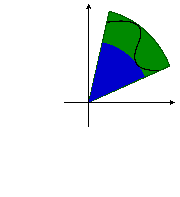
\includegraphics[scale=2.5]{images/sector.pdf}
    % \caption{$|\Delta|\inf\Delta g$ и $|\Delta|\sup g$}
\end{wrapfigure}

По теореме о вычислении аддитивной функции отрезка по плотности:
$$\Phi ([\alpha, \beta]) = \int_\alpha^\beta g(\varphi)d\varphi = \frac{1}{2}\int_\alpha^\beta r^2(\varphi)d\varphi$$
%</площадькриволинейногосектора1>

\begin{example}

    %<*площадькриволинейногосектора2>

    $\sphericalangle x(t), y(t)$ --- кривая в $\R^2$

    $$S=\frac{1}{2}\int_\alpha^\beta r^2(\varphi) d\varphi = \frac{1}{2}\int_{t_\alpha}^{t_\beta} r^2(\varphi(t)) d\varphi(t) = \frac{1}{2}\int_{t_\alpha}^{t_\beta} r^2(t) \varphi'(t) dt =$$
    $$= \frac{1}{2}\int_{t_\alpha}^{t_\beta} \sqrt{x^2(t) + y^2(t)}^2 \left(\arctg\frac{y(t)}{x(t)}\right)'dt =$$
    $$= \frac{1}{2}\int_{t_\alpha}^{t_\beta} \left(x^2(t) + y^2(t)\right) \frac{1}{1+\left(\frac{y(t)}{x(t)}\right)^2}\left(\frac{y(t)}{x(t)}\right)'dt =$$
    $$=\frac{1}{2}\int_{t_\alpha}^{t_\beta} \left(x^2(t) + y^2(t)\right) \frac{1}{1+\left(\frac{y(t)}{x(t)}\right)^2}\frac{y'(t)x(t)-y(t)x'(t)}{x^2(t)}dt=$$
    $$=\frac{1}{2}\int_{t_\alpha}^{t_\beta} \left(x^2(t) + y^2(t)\right) \frac{x^2(t)}{x^2(t)+y^2(t)}\frac{y'(t)x(t)-y(t)x'(t)}{x^2(t)}dt=$$
    $$=\frac{1}{2}\int\limits_{t_\alpha}^{t_\beta} \left(y'(t)x(t)-y(t)x'(t)\right)dt$$
    %</площадькриволинейногосектора2>
    $x:=\sin t, y:=\cos t$
    $$S=\frac{1}{2}\int\limits_{0}^{\frac{\pi}{2}}-\sin^2 t -\cos^2 t  dt = -\frac{\pi}{4} \text{ --- проблема, отрицательная площадь}$$

\end{example}

\section{Выпуклость функций}

$\forall z\in[x,y] \ \ \exists \alpha\in[0,1]: z = \alpha x + (1-\alpha) y$

$\alpha$ --- доля отрезка $zy$ от $xy$, т.е. $\alpha=\frac{|zy|}{|xy|}$

\begin{definition}
    %<*выпуклаяфункция>
    $f:\langle a,b\rangle\to\R$ --- \textbf{выпуклая}
    $$\forall x,y\in\langle a,b\rangle \quad \forall \alpha\in[0,1] \quad f(\alpha x + (1-\alpha)y)\leq \alpha f(x) + (1-\alpha)f(y)$$
    %</выпуклаяфункция>
\end{definition}

%<*выпуклаяфункцияremark>
\begin{remark}

    $f$ --- выпуклая $\Leftrightarrow$ всякая хорда графика $f$ расположена ``выше'' графика \textit{(нестрого выше)} $\Leftrightarrow$ $\text{НГ}(f, \langle a,b\rangle)\{(x,y) : x\in\langle a,b\rangle \ \ y\geq f(x)\}$
\end{remark}
%</выпуклаяфункцияremark>

Выпуклый = выпуклый вниз; вогнутый = выпуклый вверх

\begin{definition}
    %<*строговыпуклаяфункция>
    $f:\langle a,b\rangle\to\R$ --- \textbf{строго выпуклая}
    $$\forall x,y\in\langle a,b\rangle \quad \forall \alpha\in(0,1) \quad f(\alpha x + (1-\alpha)y)< \alpha f(x) + (1-\alpha)f(y)$$
    %</строговыпуклаяфункция>
\end{definition}

\begin{definition}
    %<*выпуклоемножество>
    $A\subset \R^m$ --- \textbf{выпуклое множество в $\R^m$}, если
    $$\forall x,y\in A, \alpha\in[0,1] \quad \alpha x + (1-\alpha) y \in A$$
    \textcolor{red}{Это определение с вики}
    %</выпуклоемножество>
\end{definition}

\begin{definition}
    %<*надграфик>
    \textbf{Надграфик} функции $f:\langle a,b\rangle\to \R$ это множество $\{(x, y)\ |\ x\in\langle a,b\rangle, y\ge f(x)\}$
    %</надграфик>
\end{definition}

\begin{lemma}
    о трех хордах

    %<*леммаотреххордах>
    $f:\langle a,b\rangle\to\R$. Тогда эквивалентны следующие утверждения:
    \begin{enumerate}
        \item $f$ --- вып. $\langle a,b\rangle$
        \item $\forall x_1,x_2,x_3\in\langle a,b\rangle \ \ x_1<x_2<x_3 \quad \frac{f(x_2)-f(x_1)}{x_2-x_1}\leq\frac{f(x_3)-f(x_1)}{x_3-x_1}\leq\frac{f(x_3)-f(x_2)}{x_3-x_2}$
    \end{enumerate}
    %</леммаотреххордах>
\end{lemma}
%<*леммаотреххордахproof>
\begin{proof}
    Левое $\Leftrightarrow f(x_2)(x_3-x_1)\leq f(x_3)(x_2-x_1)+f(x_1)(x_3-x_1-(x_2-x_1))$

    $$f\left(x_3\frac{x_2-x_1}{x_3-x_1}+x_1\frac{x_3-x_2}{x_3-x_1}\right)=f(x_2)\leq f(x_3)\frac{x_2-x_1}{x_3-x_1}+f(x_1)\frac{x_3-x_2}{x_3-x_1}$$
\end{proof}
%</леммаотреххордахproof>
\begin{remark}
    Если $f$ --- строго выпуклая, то в лемме оба неравенства строгие.
\end{remark}

\begin{theorem}
    об одностронней дифференциируемости выпуклой функции.

    %<*ободностроннейдифференциируемостивыпуклойфункции>
    $f$ --- вып. $\langle a,b\rangle$. Тогда $\forall x\in(a,b) \ \ \exists f_+'(x), f_-'(x)$ и $\forall x_1, x_2\in(a,b), x_1<x_2$
    $$f_-'(x_1)\leq f_+'(x_1)\leq \frac{f(x_2)-f(x_1)}{x_2-x_1}\leq f_-'(x_2)$$
    %</ободностроннейдифференциируемостивыпуклойфункции>
\end{theorem}
%<*ободностроннейдифференциируемостивыпуклойфункцииproof>
\begin{proof}
    $f_+'(x_1)=\lim\limits_{x\to x_1+0}\frac{f(x)-f(x_1)}{x-x_1}$ --- монотонно убывающая функция от $x$

    Фиксируем $x_0<x_1$. По лемме о трех хордах $\frac{f(x_0)-f(x_1)}{x_0-x_1}\leq\frac{f(x)-f(x_1)}{x-x_1}$
\end{proof}
%</ободностроннейдифференциируемостивыпуклойфункцииproof>

\begin{corollary}
    $f$ --- вып. на $\langle a,b\rangle \Rightarrow f$ непр. на $(a,b)$
    $$\lim\limits_{x\to x_0+0}f(x)=f(x_0)$$
\end{corollary}

\begin{theorem}
    выпуклость в терминах касательных

    %<*описаниевыпуклостиспомощьюкасательных>
    $f$ --- вып. на $\langle a,b\rangle$. Тогда график $f$ расположен не ниже любой касательной

    т.е. $\forall x, x_0 \quad f(x)\geq f(x_0)+f'(x_0)(x-x_0)$
    %</описаниевыпуклостиспомощьюкасательных>
\end{theorem}

%<*описаниевыпуклостиспомощьюкасательныхproof>
\begin{proof}
    ``$\Rightarrow$''

    Если $x>x_0 \quad f'(x_0)\leq\frac{f(x)-f(x_0)}{x-x_0}$, это неравенство 2. из предыдущей теоремы

    $x<x_0$ аналогично

    ``$\Leftarrow$'' фиксируем $x_0$. Берем $x_1<x_0<x_2$

    $f(x_1)\geq f(x_0)+f'(x_0)(x_1-x_0)$; $f(x_2)\geq f(x_0)+f'(x_0)(x_2-x_0)$, т.е. $\frac{f(x_1)-f(x_0)}{x_1-x_0}\leq f'(x_0)\leq \frac{f(x_2)-f(x_0)}{x_2-x_0}$. Это верно по лемме.
\end{proof}
%</описаниевыпуклостиспомощьюкасательныхproof>

\begin{definition}
    %<*опорнаяпрямая>
    $A\subset \R^2$ --- вып. $l\subset \R^2$ --- прямая

    $l$ --- \textbf{опорная прямая} к $A$, если:
    \begin{enumerate}
        \item $A$ содержится в одной полуплоскости относительно $l$
        \item $l\cap A\not=\text{\O}$
    \end{enumerate}
    %</опорнаяпрямая>
\end{definition}

\begin{theorem}
    дифференциальный критерий выпуклости

    %<*дифференциальныйкритерийвыпуклости>
    \begin{enumerate}
        \item $f:\langle a,b\rangle\to\R$, дифф. в $(a,b)$

              Тогда $f$ --- вып. $\Rightarrow f'$ возр. на $(a,b)$

              Если $f$ --- строго выпуклая $\Rightarrow$ $f'$ строго возрастает

        \item $f:\langle a,b\rangle\to\R$, дважды дифф. на $(a,b)$

              $f$ --- вып. $\Leftrightarrow f''\geq0$ на $(a,b)$
              \begin{enumerate}
                  \item ``$\Rightarrow$'' $f_+'(x_1)\leq f_-'(x_2) \quad (x_1<x_2)$

                        ``$\Leftarrow$'' $?f$ вып. $\frac{f(x_2)-f(x_1)}{x_2-x_1}=f'(c_1)<f'(c_2)=\frac{f(x_3)-f(x_2)}{x_3-x_2}$

                        Теперь утверждение 2. очевидно.
              \end{enumerate}
    \end{enumerate}
    %</дифференциальныйкритерийвыпуклости>
\end{theorem}

\begin{remark}
    %<*следствиеоточкахразрывапроизводнойвыпуклойфункции>
    $f:\langle a,b\rangle\to\R$ --- вып.

    Тогда $f$ --- дифф. на $(a,b)$ за исключением, может быть, счетного множества точек.
    %</следствиеоточкахразрывапроизводнойвыпуклойфункции>
\end{remark}

%<*следствиеоточкахразрывапроизводнойвыпуклойфункцииproof>
\begin{proof}
    $\forall x \ \ \exists f_+'(x), f_-'(x)$

    $f_\pm'$ возрастает

    $f_-'(x)=f_+'(x)\Rightarrow f$ дифф. в $x$

    $f_-'(x)<f_+'(x)\Rightarrow f$ не дифф. в $x$

    Тогда $x$ --- точка скачка для $f_+', f_-'$, их НБСЧ, т.к. $f^+$ и $f^-$ возрастают.
\end{proof}
%</следствиеоточкахразрывапроизводнойвыпуклойфункцииproof>

\begin{example}
    %<*изопериметрическоенеравенство>
    Изопериметрическое неравенство

    $G\subset\R^2$ --- выпуклое замкнутое множество (ограниченное)

    $diam G = \sup\{\rho(x,y), \ x,y\in G\}$

    $diam G \leq 1$

    Тогда $\sigma(G)\leq \frac{\pi}{4}$
    %</изопериметрическоенеравенство>

    %<*изопериметрическоенеравенствоproof>
    \begin{proof}
        Пойдём от некоторой точки на границе $G$ под углом $\varphi$ внутрь фигуры по прямой. В какой-то момент мы встретим другую граничную точку. Назовем этот процесс $r(\varphi)$ \textit{(возвращает длину пути)}. Очевидно, что $r^2(\varphi)+r^2(\varphi-\frac{\pi}{2})\leq (diam G)^2\leq 1$

        $$\sigma(G)=\frac{1}{2}\int\limits_{-\frac{\pi}{2}}^{\frac{\pi}{2}} r^2(\varphi)d\varphi = \frac{1}{2}\left(\int\limits_{-\frac{\pi}{2}}^0r^2(\varphi)d\varphi + \int\limits^{\frac{\pi}{2}}_0r^2(\varphi)d\varphi\right) =$$
        $$=\frac{1}{2}\int\limits_{0}^{\frac{\pi}{2}}\left(r^2(\varphi)+r^2\left(\varphi-\frac{\pi}{2}\right)\right)d\varphi\le \frac{1}{2}\int\limits_{0}^{\frac{\pi}{2}}1 d\varphi=\frac{\pi}{4}$$
    \end{proof}
    %</изопериметрическоенеравенствоproof>
\end{example}

\end{document}